\documentclass{article}
\usepackage{graphicx} % Required for inserting images
\usepackage{float}  % For wrapping text around figures
\usepackage{pgfplots}
\usepackage{amsmath} % Required for cases environment
\usepackage{mathrsfs}
\usepackage{amssymb} % For \mathbb
\usepackage{listings}
\usepackage{xcolor}

% Bibliography: classic BibTeX with the IEEEtran style (see Sources.bib and
% \bibliography near the end of the document).

\pgfplotsset{compat=1.18} % Ensure latest features

\graphicspath{ {./Figures/} }

\usepackage[a4paper, margin=1in]{geometry}
% Define style
\lstset{
    basicstyle=\ttfamily\small,
    keywordstyle=\color{blue},
    stringstyle=\color{red},
    commentstyle=\color{green!50!black},
    showstringspaces=false,
    breaklines=true
}

\title{BoMu: A Resistively-Loaded NMOS Differential Pair\\ Design \& Sizing (SKY130A, TinyTapeout)}
\author{Mathew Hanson}
\date{August 2026}

\begin{document}

\maketitle

\section{Introduction}
\texttt{BoMu} is a single-stage differential amplifier built from a resistively-loaded
NMOS source-coupled pair, designed for the SKY130A PDK and open-source TinyTapeout flow. Two
matched NMOS devices ($M_1$, $M_2$) share a tail sink of $2I_D$, and each drain is
pulled to the $1.2V$ supply through a load resistor $R_D$. The amplifier output is taken
differentially across the drains, $v_{od}=v(\text{voutp})-v(\text{voutn})$. A
floating differential source $\pm v_{sd}/2$ on a common-mode $V_{SC}$ drives the
gates through $100\Omega$ series resistors.

The driving bandwidth constraint is that each output drives an I/O pad of
fixed $C_L=5pF$. The tail sink is realised on-chip as a simple current mirror
(Section~\ref{sec:tailbias}) with a $200mV$ compliance budget. The flow is fully
open-source (\texttt{xschem}, \texttt{ngspice}, \texttt{magic}/\texttt{klayout});
devices are sized by a $g_m/I_D$ methodology~\cite{Jespers_gmID} from measured
current-density and speed data rather than an assumed square-law constant, and the
small-signal results are standard~\cite{Razavi_AnalogCMOS}.

\subsection{Net identities}
With the sign convention $M_1$ gate $=$ \texttt{vinp} $\rightarrow$ drain $=$
\texttt{voutn}, and $M_2$ gate $=$ \texttt{vinn} $\rightarrow$ drain $=$ \texttt{voutp},
the differential output $v_{od}=v(\text{voutp})-v(\text{voutn})$ has positive
gain with respect to the differential input $v_{id}=\text{vinp}-\text{vinn}$. The two
half-circuits are identical by matching, so the analysis is done on a single common-source
half-circuit and the differential result follows directly.

\section{Specifications}
\label{sec:specs}
The target specifications, and recommended design parameters, are collected
in Table~\ref{tab:specs}.

\begin{table}[H]
    \centering
    \caption{Design targets and recommended parameters.}
    \label{tab:specs}
    \begin{tabular}{l|c|c} \hline
        \textbf{Parameter} & \textbf{Value} & \textbf{Units} \\ \hline
        Small-signal bandwidth $f_{-3dB}$ & $150$ & $MHz$ \\ \hline
        Differential DC gain $A_{v0}$ & $10$ & $dB$ \\ \hline
        Differential output swing $v_{od}$ & $400$ & $mV_{pp}$ \\ \hline
        Channel length $L$ & $0.15$ & $\mu m$ \\ \hline \hline
        Supply $V_{DD}$ & $1.2$ & $V$ (fixed) \\ \hline
        Pad load $C_L$ (each output) & $5$ & $pF$ (fixed) \\ \hline
        Tail-sink compliance budget & $200$ & $mV$ (fixed) \\ \hline
    \end{tabular}
\end{table}

\section{First-Order Hand Design}
\label{sec:hand}
The design proceeds as follows: the fixed pad capacitance and the bandwidth target set the
load resistor, the gain target then sets the required transconductance, and a chosen
inversion level ($g_m/I_D$) fixes the bias current.

\paragraph{Load resistor from bandwidth.} The dominant pole sits at the output node,
formed by the load resistance working into the fixed $C_L$. Ignoring the device output
resistance for the moment,
\begin{equation}
    R_D \;=\; \frac{1}{2\pi f_{-3dB} C_L}
           \;=\; \frac{1}{2\pi(150\mathrm{MHz})(5\mathrm{pF})}
           \;\approx\; 212\Omega .
    \label{eq:RD}
\end{equation}

\paragraph{Transconductance from gain.} The differential (half-circuit) gain of a
resistively-loaded pair is
\begin{equation}
    A_{v0} \;=\; g_m(R_D \| r_o) \;\xrightarrow{\;r_o \gg R_D\;}\; g_m R_D .
    \label{eq:gain}
\end{equation}
With $A_{v0}=10\mathrm{dB}=3.162\mathrm{V/V}$ and Eq.~\eqref{eq:RD},
\begin{equation}
    g_m \;=\; \frac{A_{v0}}{R_D} \;=\; \frac{3.162}{212\Omega} \;\approx\; 14.9\mathrm{mS}.
    \label{eq:gm}
\end{equation}

\paragraph{Bias current from $g_m/I_D$.} Choosing a moderate-inversion
$g_m/I_D = 15\mathrm{V^{-1}}$ (a balance of device area, $r_o$, and speed at this
minimum length) fixes the per-branch current and the tail current,
\begin{equation}
    I_D \;=\; \frac{g_m}{(g_m/I_D)} \;=\; \frac{14.9\,\mathrm{mS}}{15} \;\approx\; 0.99\mathrm{mA},
    \qquad I_{\text{tail}} = 2I_D \approx 2\mathrm{mA}.
\end{equation}

\paragraph{Swing and headroom.} A $400mV_{pp}$ differential swing corresponds to
a single-ended peak of $v_{od}/4 = 100mV$ about each drain's DC level
$V_D = V_{DD}-I_D R_D \approx 0.99\,V$. Two conditions must hold: the bias drop must be
large enough to source the swing, $I_D R_D > 100mV$ ($R_D = 212mV$ is ample), and the
device must remain saturated at the bottom of the swing,
$V_{D,\min}-(V_S+V_{ov}) > 0$, where $V_S$ is the tail-node voltage held at or above the
$200\,mV$ compliance budget. Both are comfortably satisfied because $R_D$ is small and the
supply headroom is large.

\section{$g_m/I_D$ Sizing Flow}
\label{sec:flow}
Equations~\eqref{eq:RD}--\eqref{eq:gm} fix $R_D$ and the required $g_m$. The $g_m/I_D$
method then turns the chosen inversion level into a physical width. A unit device is
characterised over $V_{GS}$ at fixed $(V_{SB},V_{DS})$ to build a lookup grid returning,
for any $g_m/I_D$, the current density $J_D$ (=$I_D/W$), the intrinsic gain $g_m r_o$, and
the transit frequency $f_T$. The width then follows as
\begin{equation}
    W \;=\; \frac{I_D}{J_D(g_m/I_D,\,V_{SB},\,V_{DS})} .
    \label{eq:W}
\end{equation}
This is implemented in \texttt{sim/sizing.py (worksheet)}, which references the \texttt{extern/sky130A-gmid} 
lookup grid (a git submodule). The script takes a \texttt{DESIGN} dict (targets $+$ the two free
knobs, $g_m/I_D$ and $V_S$), prints the worksheet of
Table~\ref{tab:sizing}, and with \texttt{--spice} generates a differential-pair deck,
runs \texttt{ngspice}, and reports predicted-versus-SPICE side by side
(Table~\ref{tab:verify}).

\begin{table}[H]
    \centering
    \caption{Sizing worksheet at example operating point ($g_m/I_D=15$,
             $V_S=0.30\,V$, $L=0.15\,\mu m$, SKY130A \texttt{nfet\_01v8\_lvt}).}
    \label{tab:sizing}
    \begin{tabular}{l|c|c} \hline
        \textbf{Quantity} & \textbf{Value} & \textbf{Units} \\ \hline
        $R_D$ (from BW) & $212$ & $\Omega$ \\ \hline
        $g_m$ required (from gain) & $14.9$ & $mS$ \\ \hline
        $I_D$ / $I_{\text{tail}}$ & $0.99$ / $1.99$ & $mA$ \\ \hline
        $V_{ov}=2/(g_m/I_D)$ & $0.133$ & $V$ \\ \hline
        current density $J_D$ & $14.6$ & $\mu A/\mu m$ \\ \hline
        width $W$ (per device) & $68.0$ & $\mu m$ \\ \hline
        output resistance $r_o$ & $941$ & $\Omega$ \\ \hline
        intrinsic gain $g_m r_o$ & $14.0$ & --- \\ \hline
        transit frequency $f_T$ & $51.3$ & $GHz$ \\ \hline
        bias nodes $V_D$ / $V_{DS}$ & $0.989$ / $0.689$ & $V$ \\ \hline
        power $V_{DD}\!\cdot\!I_{\text{tail}}$ & $2.38$ & $mW$ \\ \hline
    \end{tabular}
\end{table}

\section{The $r_o$-Limited Gain}
\label{sec:ro}
Equation~\eqref{eq:gain} assumed $r_o \gg R_D$, but at minimum length this does not hold.
The lookup returns $r_o \approx 941\Omega$ at $g_m/I_D = 15$, so the effective
load is
\begin{equation}
    R_L \;=\; R_D \| r_o \;=\; 212 \| 941 \;\approx\; 173\Omega,
\end{equation}
and the realised gain and bandwidth become
\begin{equation}
    A_{v0} = g_m R_L \approx 2.58\ \mathrm{V/V}\ (8.23\mathrm{dB}),
    \qquad
    f_{-3dB} = \frac{1}{2\pi R_L C_L} \approx 184\mathrm{MHz}.
\end{equation}
Because $R_D$ is pinned at $212\,\Omega$ by the fixed $C_L$ and the bandwidth target
(Eq.~\eqref{eq:RD}), and $r_o$ at this length is comparable to $R_D$, the gain $+$ BW targets are
in competing: the finite $r_o$ pulls the gain down to $\sim 8.2dB$ while pushing the
bandwidth up past $150MHz$. A single resistively-loaded stage at
$L=0.15\mu m$ cannot simultaneously meet $10dB$ and $150MHz$ for the selected $R_D$.

Figure~\ref{fig:tradeoff} makes this concrete: sweeping the inversion level with $g_m$
held at the gain-target value ($14.9\,mS$), the realised gain plateaus near
$8.3dB$ and never reaches $10\,dB$. At $L=0.15\,\mu m$ the intrinsic $g_m r_o$ is
simply too small for $r_o$ to dominate $R_D$, regardless of bias.

\begin{figure}[H]
\centering
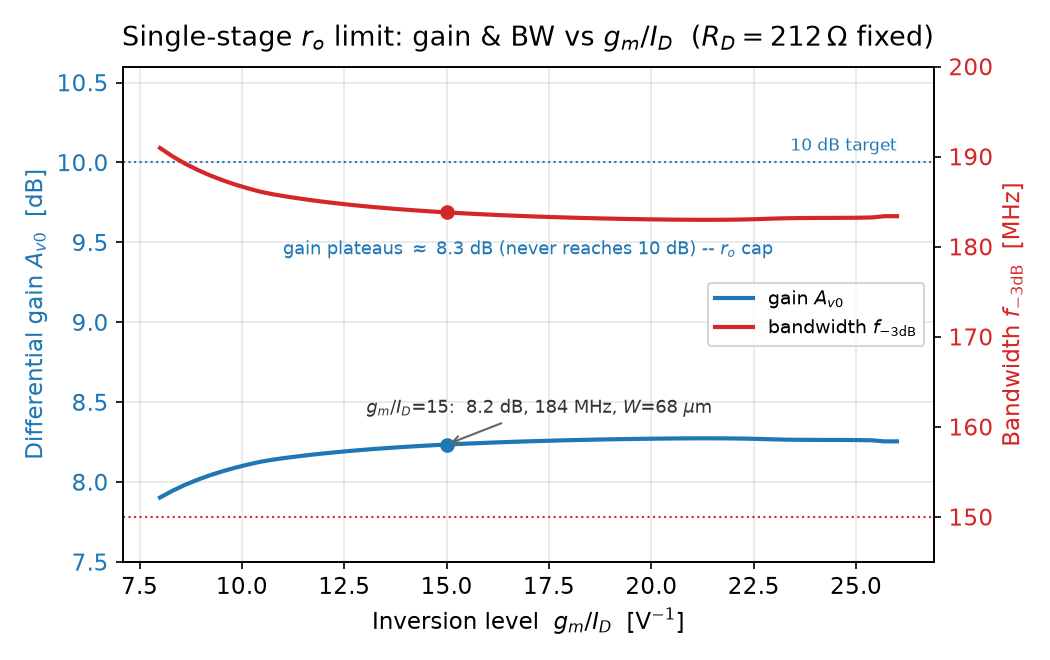
\includegraphics[width=12cm]{Figures/bomu_gain_bw_tradeoff.png}
\caption{Gain and bandwidth versus inversion level $g_m/I_D$, with $g_m$ fixed at the
$14.9mS$ the $10dB$ target requires and $R_D=212\Omega$ pinned by the bandwidth.
The gain plateaus near $8.3dB$}
\label{fig:tradeoff}
\end{figure}

\section{SPICE Verification (SKY130A, tt corner)}
\label{sec:spice}
The self-contained differential AC testbench \texttt{sim/tb\_ac.spice} (floating
$\pm v_{sd}/2$ drive, $100\Omega$ gate resistors, ideal $2I_D$ tail sink, $5pF$
pad caps) exercises the design under \texttt{ngspice} with the SKY130A \texttt{tt}
models. The hand-calculations track SPICE closely as shown in Table~\ref{tab:verify}.
Particularly, the $R_D\|r_o$ gain estimate of Section~\ref{sec:ro} reproduce the
simulated gain to within $0.01dB$, confirming the $r_o$-limited result is real.

\begin{table}[H]
    \centering
    \caption{Predicted (hand-calc) versus SPICE at the sized operating point
             ($W=68\mu m$, $g_m/I_D=15$).}
    \label{tab:verify}
    \begin{tabular}{l|c|c|c} \hline
        \textbf{Quantity} & \textbf{Predicted} & \textbf{SPICE} & \textbf{Units} \\ \hline
        Tail current $I_{\text{tail}}$ & $1987$ & $1987$ & $\mu A$ \\ \hline
        $g_m$ per device & $14.9$ & $14.85$ & $mS$ \\ \hline
        Tail-node voltage $V_S$ & $0.30$ & $0.205$ & $V$ \\ \hline
        Differential gain $A_{v0}$ & $8.23$ & $8.24$ & $dB$ \\ \hline
        Bandwidth $f_{-3dB}$ & $183.8$ & $177.8$ & $MHz$ \\ \hline
    \end{tabular}
\end{table}

\noindent The simulated response (Figure~\ref{fig:ac}) is a flat $\sim8.2dB$
passband rolling off at the single output pole. The responce is both below the $10dB$ gain
target and above the $150MHz$ bandwidth target.
The tail node settles at $205mV$ (just above the $200mV$) and the drain DC operating point 
of $0.988V$ matches $V_{DD}-I_D R_D$ exactly.

\begin{figure}[H]
\centering
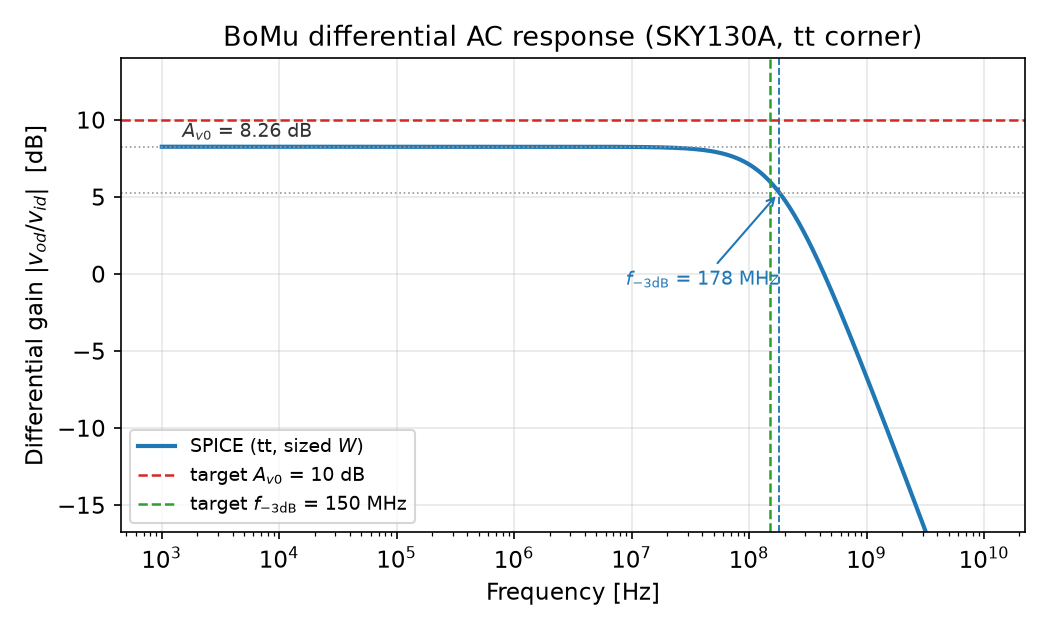
\includegraphics[width=12cm]{Figures/bomu_ac_response.png}
\caption{Differential AC response from \texttt{sim/tb\_ac.spice} (SKY130A, \texttt{tt},
sized $W=68\mu m$).}
\label{fig:ac}
\end{figure}

\section{Design-Space Sweeps and the Gain--Bandwidth Limit}
\label{sec:sweeps}
Section~\ref{sec:ro} showed that at the chosen $R_D=212\Omega$, the finite $r_o$
leaves the gain short and the bandwidth long. This section sweeps $R_D$ and $L$ to map the achievable
space.

\subsection{$R_D$: trading gain for bandwidth at constant $g_m/(2\pi C_L)$}
For a single output pole the gain--bandwidth product is
\begin{equation}
    A_{v0}\cdot f_{-3dB}
    = g_m(R_D\|r_o)\cdot\frac{1}{2\pi(R_D\|r_o)C_L}
    = \frac{g_m}{2\pi C_L},
    \label{eq:gbw}
\end{equation}
With $g_m=14.9mS$ and $C_L=5pF$ this
ideal product is $474MHz$. Sweeping $R_D$ (Figure~\ref{fig:sweeprd}) therefore slides
the design along this fixed hyperbola. A larger $R_D$ buys gain at the cost of
bandwidth. This sweep is at constant power, since $R_D$ draws no bias current.

\begin{figure}[H]
\centering
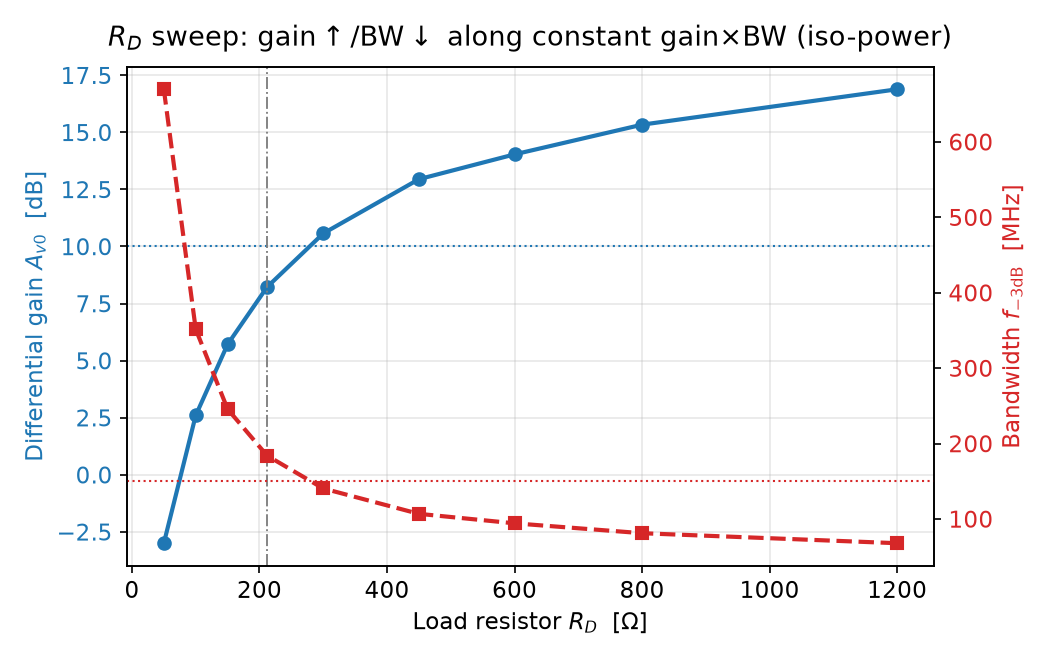
\includegraphics[width=12cm]{Figures/bomu_sweep_rd.png}
\caption{$R_D$ sweep (iso-power $2.38mW$): gain rises and bandwidth falls along
the constant $g_m/(2\pi C_L)$ product. Dotted lines are the $10dB$ and $150MHz$
targets.}
\label{fig:sweeprd}
\end{figure}

Channel length was also swept in an attempt to recover additional gain. Longer $L$ raises $r_o$, so
$R_D\|r_o\to R_D$ and the gain climbs toward the ideal $g_m R_D$ at constant power
(the current is unchanged, $W\propto L$ to hold the inversion level). The recovery is
modest and saturating: $8.2dB$ at $L=0.15\mu m$ up to only $\approx9.1dB$ by
$L=0.6\mu m$, which was still short of the $10dB$ target confirming the $r_o$-limited ceiling of
Section~\ref{sec:ro}. Length trades area for a fraction of the missing gain but does
not, on its own, reach the target.

\subsection{Is $R_D\approx280\,\Omega$ feasible for $10\,dB$ and $150\,MHz$?}
The two targets have product $3.162\times150MHz=474MHz$, which is exactly the ideal
GBW of Eq.~\eqref{eq:gbw}. The specification therefore sits right on the
single-stage limit, reachable only if the realised product equals the ideal. It does
not: second-order gate/Miller poles pull the SPICE gain--bandwidth product down to
$\approx467MHz$, about $1.5\%$ short. Table~\ref{tab:rdbracket} brackets $R_D$ in SPICE
(\texttt{tt}, $L=0.15$, $W=68$), note no value of $R_D$ has sufficient GBW product at the chosen $g_m$.

\begin{table}[H]
    \centering
    \caption{$R_D$ bracket in SPICE.}
    \label{tab:rdbracket}
    \begin{tabular}{c|c|c|c} \hline
        $R_D$ [$\Omega$] & $A_{v0}$ [dB] & $f_{-3dB}$ [MHz] & GBW [MHz] \\ \hline
        220 & 8.49  & 175.8 & 468 \\ \hline
        250 & 9.37  & 158.7 & 467 \\ \hline
        265 & 9.76  & \textbf{151.7} & 467 \\ \hline
        280 & \textbf{10.13} & 145.4 & 467 \\ \hline
        300 & 10.58 & 137.9 & 466 \\ \hline
    \end{tabular}
\end{table}

So $R_D\approx280\Omega$ is a close but still not a feasible solution: the gain
passes ($10.13dB$) but the bandwidth is $145MHz$ ($\sim3\%$ low). Moving to
$R_D=265\Omega$ recovers bandwidth to $152MHz$ but drops the gain to $9.76dB$. The $A_{v0}=10dB$
crossover lands at $R_D\approx277\Omega$ with only $f_{-3dB}\approx148MHz$. The design
lands within $\sim2$--$3\%$ of both but meets neither pair simultaneously, with no margin. 
Considering this is the nominal \texttt{tt}/$27^\circ$C case (slow corners erode $g_m$, and
$V_{tail}$ sits at the $0.20\,V$ compliance edge in this $R_D$ range), a small margin will be require
to meet the design targets after parasitic extraction. Closing the last
few percent requires more GBW which can be achieved with a slighty higher $g_m$ (more current/power).

\subsection{Meeting both specs: a small $g_m$ increase}
\label{sec:hit}
Because the realised GBW scales with $g_m$ (Eq.~\eqref{eq:gbw}), the $\sim1.5\%$
shortfall is closed by a comparably small increase in $g_m$. Holding $g_m/I_D=15$ and $L=0.15\mu m$, raising $g_m$ from
$14.9$ to $16.0mS$ (widening the pair to $W=73\mu m$ and the tail to
$I_{tail}=2.13mA$) lifts the realised gain--bandwidth product to $\approx500MHz$,
clearing the $474MHz$ the pair requires. Re-centring the load at $R_D=262\Omega$ then
lands both targets with margin (Table~\ref{tab:hit}): $A_{v0}=10.15dB$ and
$f_{-3dB}=155.5MHz$ at $2.56mW$ --- a $7.6\%$ power increase over the $2.38mW$
baseline. The tail node sits at $0.218V$ (with $V_{SC}=0.92V$), clear of the
$0.20V$ compliance budget.

\begin{table}[H]
    \centering
    \caption{Closing the GBW gap with a $g_m$ increase, SPICE
             \texttt{tt}, $L=0.15\mu m$, $g_m/I_D=15$.}
    \label{tab:hit}
    \begin{tabular}{c|c|c|c|c|c} \hline
        $g_m$ [mS] & $W$ [$\mu$m] & $R_D$ [$\Omega$] & $A_{v0}$ [dB] & $f_{-3dB}$ [MHz] & $P$ [mW] \\ \hline
        14.9 (base) & 68 & 212 & 8.24 & 178.0 & 2.38 \\ \hline
        15.6 & 71 & 272 & 10.23 & 150.2 & 2.50 \\ \hline
        \textbf{16.0} & \textbf{73} & \textbf{262} & \textbf{10.15} & \textbf{155.5} & \textbf{2.56} \\ \hline
        16.0 & 73 & 272 & 10.40 & 151.1 & 2.56 \\ \hline
    \end{tabular}
\end{table}

The bolded row above meets both specifications. The margins ($+0.15dB$, $+5.5MHz$) are
comfortable at nominal \texttt{tt}/$27^\circ$C but modest. A slow/hot corner erodes
$g_m$, and layout parasitics will erode the bandwidth further.
Section~\ref{sec:parasitic} addresses this directly, sizing a small additional current
margin against those parasitics to fix the final operating point.

\subsection{Layout-parasitic headroom and the pre-layout operating point}
\label{sec:parasitic}
The $g_m=16mS$ point marginally meets both targets ($f_{-3dB}$ is only $5.5MHz$ over
target), and layout will add output-node capacitance (drain-junction $C_{db}$ plus pad 
interconnect) on top of the fixed $5pF$.
Since $f_{-3dB}=1/(2\pi R_L C_{tot})$ decreases with total capacitance while the DC gain
$g_m R_L$ remains unaffected, only the bandwidth spec is exposed. The remedy is a small
$\sim7\%$ $g_m$ margin: widening the pair to $W=78\mu m$ ($I_{tail}=2.28mA$) and
re-centring $R_D=245\Omega$ lifts the nominal bandwidth to $166MHz$ at
$10.16dB$ / $2.74mW$, holding both specs past $500fF$ of added per-output
capacitance.

\subsection{Tail-current mirror and input common-mode}
\label{sec:tailbias}
The ideal tail sink is realised on-chip as a simple two-transistor
resistor-programmed NMOS mirror, kept fully internal. A cascode/Wilson mirror needs
$V_{GS}+V_{DS,sat}\gtrsim0.5V$ of compliance, far above the tail budget, so only a
simple mirror fits. The $0.218V$ tail of the sizing above is too tight for a
$2.28mA$ sink, but the pair has abundant unused $V_{DS}$ (drains at $0.9V$,
sources at the tail): raising the input common-mode from $V_{SC}=0.92$ to $1.05V$
lifts the tail to $\approx0.33V$, putting the mirror in clean saturation with a
device roughly half the width. The $400mV_{pp}$ swing survives (lowest single-ended
output $0.82V$, still $0.32V$ above the saturation floor).

The mirror uses standard-$V_T$ \texttt{nfet\_01v8} devices at $L=0.5\mu m$: output
$M_3=W80\mu m/nf8$, reference $M_4=W10\mu m/nf1$, ratio $N=8$, so the reference
leg draws only $I_{tail}/8\approx0.285mA$ through $R_{ref}\approx745\Omega$ from
$V_{DD}$. An integrated simulation (\texttt{sim/bias.py verify}) with the real
mirror replacing the ideal sink closes the operating point and leaves the
differential spec untouched (Table~\ref{tab:mirror}): at $R_{ref}=745\Omega$ the
tail settles at $0.331V$, $I_{tail}=2.28mA$, $A_{v0}=10.13dB$,
$f_{-3dB}=167MHz$. The gain only degraded by $0.035dB$ from the ideal source, as the
mirror's finite $r_{out}$ lands on the common-mode path ($\text{CMRR}\approx30dB$),
not the differential one. Power is $3.08mW$. Because the reference is a plain
resistor from $V_{DD}$, $I_{tail}$ tracks supply/temperature/process --- the axis
that dominates the PVT sweep of Section~\ref{sec:corners}. The mirror is folded
into \texttt{ip/bomu.sch} ($M_3$/$M_4$, $R_{ref}$).

\begin{table}[H]
    \centering
    \caption{Integrated verification (\texttt{sim/bias.py verify}): BoMu with the real
             tail mirror ($W_{out}=80$, $W_{ref}=10$, $L=0.5$, $N=8$), sweeping the
             programming resistor. $V_{SC}=1.052V$.}
    \label{tab:mirror}
    \begin{tabular}{c|c|c|c|c} \hline
        $R_{ref}$ [$\Omega$] & $V_{tail}$ [V] & $I_{tail}$ [mA] & $A_{v0}$ [dB] & $f_{-3dB}$ [MHz] \\ \hline
        720 & 0.330 & 2.322 & 10.19 & 167.5 \\ \hline
        745 & 0.331 & 2.284 & 10.13 & 167.1 \\ \hline
        760 & 0.332 & 2.261 & 10.09 & 166.8 \\ \hline
    \end{tabular}
\end{table}

\section{PVT Corner Sign-off and the Final Re-size}
\label{sec:corners}
The operating point of Sections~\ref{sec:parasitic}--\ref{sec:tailbias}
($g_m=17.1mS$, $W=78\mu m$, $R_D=245\Omega$) meets both specifications, but
only at the nominal \texttt{tt}/$27^\circ$C/$1.20V$ point. A proper sign-off requires the
full process--voltage--temperature (PVT) check. The pair is swept over a
$63$-point grid --- seven process corners
$\{\texttt{tt},\texttt{ss},\texttt{ff},\texttt{ss\_ll},\texttt{ss\_hh},
\texttt{ff\_ll},\texttt{ff\_hh}\}$ (the \texttt{\_ll}/\texttt{\_hh} suffixes are
the poly-resistor process skews) crossed with $T\in\{0,27,70\}^\circ$C and
$V_{DD}\in\{1.14,1.20,1.26\}V$ ($\pm5\%$) --- driven off the extracted schematic netlist
by \texttt{sim/corners.py}, so the loads are the actual
\texttt{res\_high\_po} devices (which track the resistor corner) and the tail is
the real mirror (not the idealised $R_D=245$/$R_{ref}=745$ of the testbench).

At $W=78\mu m$ the sweep fails PVT badly, only $\sim12/63$ corners pass. The failure
is structural, not a trim: the gain--bandwidth wall $A_{v0}\!\cdot\!f_{-3dB}
=g_m/(2\pi C_L)$ of Eq.~\eqref{eq:gbw}, which nominal clears by only $\sim1.5\%$
while the PVT spread is far wider. Three mechanisms bind. \emph{(i)} Supply: the
simple mirror sets $I_{tail}\propto(V_{DD}-V_{GS})/R_{ref}$, so the whole
$1.14V$ column droops in $g_m$. \emph{(ii)} Temperature: hot always erodes
mobility and hence $g_m$. \emph{(iii)} The resistor corner has a more nuanced impact --- gain
$\propto R_D$ but bandwidth $\propto1/R_D$, so the \texttt{ll} skew kills gain and
the \texttt{hh} skew kills bandwidth, and no single $R_D$ centres both. An
$I_{tail}$ sweep confirms current alone cannot rescue the slow/hot/low-$R$ corner
($g_m\propto\sqrt{I_D}$: $+40\%$ current buys only $\sim1.5dB$).

Two decisions close the sign-off. First, treat $V_{DD}$ as regulated
(a positive-tolerance $1.20V$ rail), which removes the dominant supply axis.
The binding limit then becomes the low-$R$ resistor corner, whose $\sim-16\%$
spread must be covered by raw $g_m$. Second, brute-force $g_m$ by widening
the pair to $W=320\mu m$ ($nf=33$) and re-centring the loads at $R_D=193\Omega$
(a wider \texttt{res\_high\_po\_5p73} at $L=2.21\mu m$), with the mirror
programming resistor moved to $R_{ref}\approx380\Omega$
(\texttt{res\_high\_po\_2p85}, $L=1.74\mu m$) for $I_{tail}\approx2.8mA$. This
is the point folded into \texttt{ip/bomu.sch} and carried into layout.
Table~\ref{tab:finalsize} summarizes it.

\begin{table}[H]
    \centering
    \caption{Signed-off sizing (\texttt{ip/bomu.sch}).}
    \label{tab:finalsize}
    \begin{tabular}{l|c|c} \hline
        \textbf{Device} & \textbf{Sizing} & \textbf{Role} \\ \hline
        $M_1,M_2$ (pair) & \texttt{nfet\_01v8\_lvt} $W{=}320\,\mu m$, $L{=}0.15$, $nf{=}33$ & input diff pair \\ \hline
        $R_{D1},R_{D2}$ & \texttt{res\_high\_po\_5p73} $L{=}2.21\,\mu m$ ($\approx193\,\Omega$) & drain loads \\ \hline
        $M_3$ (mirror out) & \texttt{nfet\_01v8} $W{=}80\,\mu m$, $L{=}0.5$, $nf{=}8$ & tail sink ($N{=}8$) \\ \hline
        $M_4$ (mirror ref) & \texttt{nfet\_01v8} $W{=}10\,\mu m$, $L{=}0.5$, $nf{=}1$ & diode reference \\ \hline
        $R_{ref}$ & \texttt{res\_high\_po\_2p85} $L{=}1.74\,\mu m$ ($\approx380\,\Omega$) & $I_{tail}$ program \\ \hline
        $I_{tail}$ & $\approx2.8\,mA$ (regulated $1.20\,V$) & --- \\ \hline
    \end{tabular}
\end{table}

At this sizing the full $\pm5\%$ VDD grid gives $61/63$ passing corners: bandwidth now
clears $150MHz$ at every corner (worst $161MHz$ @ \texttt{ss\_hh}/$70/1.14$),
and the only two misses are marginal gain ($9.64dB$ @ \texttt{ss\_ll}/$70/1.14$
and $9.86dB$ @ \texttt{ff\_ll}/$70/1.14$), both at the simultaneous
$-5\%V_{DD}$ $+$ hot $+$ low-$R$ worst case. At the regulated $1.20V$
rail all $21$ process$\times$temperature points pass, the tightest being
\texttt{ss\_ll}/$70/1.20=10.53dB$. A VDD-margin sweep places the allowable
window at $[1.20,\ \gtrsim1.38]\,V$: the supply may rise $\sim15\%$ freely but has
essentially zero downward margin, so the $1.20V$ regulated VDD assumption is a
positive-only tolerance. The last $\sim1dB$ of gain at the low-$R$/hot
corner is what enfoces the VDD tolerance, a direct consequence of the single-stage GBW wall rather
than any bias defect.

\section{Physical Layout}
\label{sec:layout}
The \texttt{bomu} cell is drawn in \texttt{magic} on SKY130A. The overriding
layout concern for a differential pair is matching of $M_1$/$M_2$, so the
core is a common-centroid \texttt{ABBAABBA} interdigitation: a $2\times8$ array of a
\texttt{unit\_nch} cell (each $nf=4$, $W=10\mu m$, $L=0.15\mu m$, on its own
isolated diffusion island), $16$ units total ($64$ fingers), assigned to the two
halves in an alternating centroid pattern so that a linear process gradient across
the block cancels differentially.

\begin{figure}[H]
\centering
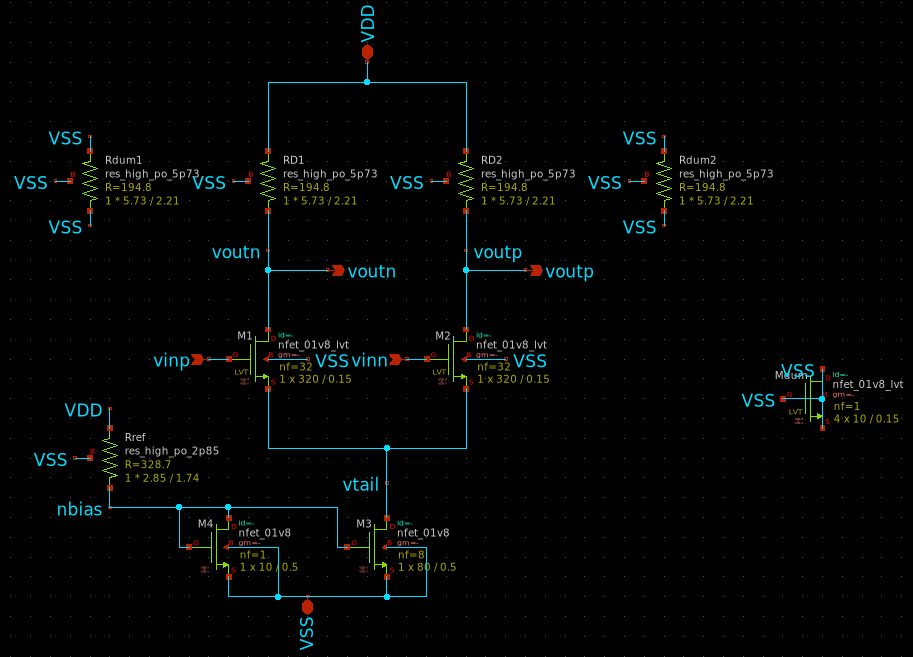
\includegraphics[width=12cm]{Figures/Xschem_Schematic.png}
\caption{The final \texttt{ip/bomu.sch} in \texttt{xschem}. This is the schematic the layout
implements and LVS-matches.}
\label{fig:sch}
\end{figure}

\paragraph{Edge dummies.} Matching is protected at the array edges by
same-width $nf=1$ dummy transistors on the left and right columns (four
dummies), which give the outermost live fingers an identical poly/diffusion
neighbourhood. A full surrounding ring of ddummy transistors was rejected as it 
would require$\sim2.6\times$ the area for
second-order benefit, since the isolated-island units already bake in first-order
length-of-diffusion matching. The dummy gates, sources and drains are all strapped
to \texttt{VSS}. The load resistors are handled the same way: the two live loads
$R_{D1}$/$R_{D2}$ (\texttt{res\_high\_po\_5p73}) are flanked by two
dummy resistors $R_{dum1}$/$R_{dum2}$ of identical geometry for etch/density
symmetry at the resistor-bank edges. These dummies are terminated to \texttt{VSS},
giving them a defined path through the p-well rather than leaving them floating.

\paragraph{Tail mirror and bias.} The mirror is laid out as a single
interdigitated row of nine \texttt{nfet\_01v8} unit fingers ($W=10\mu m$,
$L=0.5\mu m$), with the diode-connected reference $M_4$ at the row centre and the
eight $M_3$ output fingers around it (a $1$-D common-centroid, ratio $N=8$). The
programming resistor $R_{ref}$ (\texttt{res\_high\_po\_2p85}) sits beside the
mirror inside a shared bias guard ring.

\paragraph{Wells and guard rings.} Being an all-NMOS block, every sub-block (pair,
resistor bank, mirror) is wrapped in a p$^+$ guard ring tied to \texttt{VSS} with
no n-well, using a DRC-clean two-frame recipe (a wider \texttt{psubdiff}
diffusion frame with an inset \texttt{psubdiffcont} contact frame under a full
\texttt{li} cover). The six top-level ports (\texttt{vinp}, \texttt{vinn}, \texttt{voutp}, \texttt{voutn}, \texttt{VDD},
\texttt{VSS}) are brought out on \texttt{metal2} (or \texttt{metal1} for VSS) past the outer
guard ring.

\paragraph{Sign-off.} The full block (Figure~\ref{fig:layout}) is clean against
\texttt{ip/bomu.sch} (Figure~\ref{fig:sch}): \texttt{netgen} reports
\texttt{Circuits match uniquely}, \texttt{magic} geometric DRC reports $0$ errors,
and \texttt{klayout} \texttt{sky130A\_mr}
(\texttt{feol} $+$ \texttt{beol} $+$ \texttt{offgrid} $+$ \texttt{floating\_met})
reports \texttt{CLEAN}. The signed-off GDS and the LVS/DRC reports are collected in
\texttt{tapeout/} with a checksum manifest (\texttt{tapeout/SIGNOFF.md}).

\begin{figure}[H]
\centering
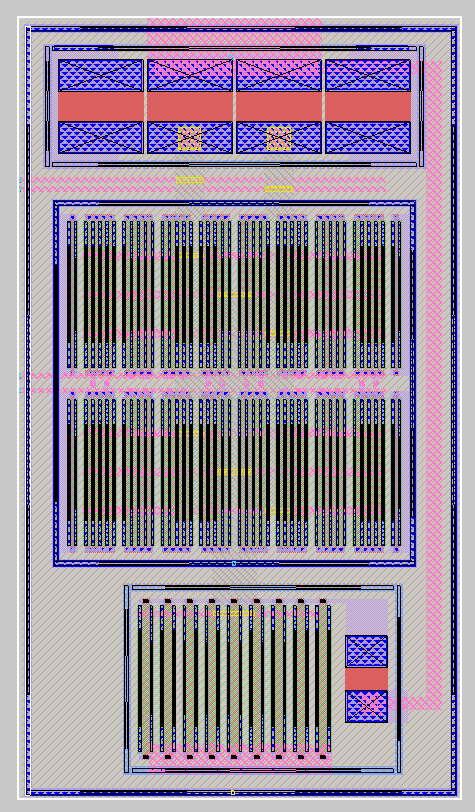
\includegraphics[width=12cm]{Figures/Magic_Layout.png}
\caption{The signed-off \texttt{bomu} layout in \texttt{magic}: the common-centroid
\texttt{ABAB} pair core with edge dummies, the flanked load-resistor bank, and the
interdigitated tail mirror, each wrapped in a \texttt{VSS}-tied p$^+$ guard ring.
DRC- and LVS-clean against the schematic of Figure~\ref{fig:sch}.}
\label{fig:layout}
\end{figure}

\section{Post-Layout Extraction (PEX/RCX) and Re-Simulation}
\label{sec:pex}
With the layout LVS/DRC-clean, the parasitics are extracted from
\texttt{layout/bomu.mag} and the PVT sweep re-run against the extracted netlist to
confirm the sign-off survives layout. Two extractions are produced (both in
\texttt{verify/}): a cap-only PEX (\texttt{ext\_pex.tcl}
$\rightarrow$ \texttt{bomu\_pex.spice}, $58$ coupling/ground capacitors) and a
full $R+C$ RCX (\texttt{ext\_rcx.tcl} $\rightarrow$ \texttt{bomu\_rcx.spice},
$75$ resistors $+$ $60$ capacitors). The RCX flow runs \texttt{magic}'s
\texttt{extresist} on the top-cell interconnect only: recursing into the PDK
device cells segfaults on the poly-resistor's internal net, and the device-internal
resistance is already in the device models, so only the \texttt{bomu} routing
needs a wire-resistance network. The extracted subckt port order
(\texttt{VSS voutn voutp VDD vinp vinn}) differs from the schematic, and the
substrate folds into \texttt{VSS} with no separate port. The PVT driver
\texttt{sim/corners.py pex} maps the DUT ports accordingly and \texttt{.include}s either
netlist, re-running the identical $63$-point grid of Section~\ref{sec:corners}.

\paragraph{Parasitic penalty.} The extracted parasitics cost bandwidth but
not gain, exactly as predicted in Section~\ref{sec:parasitic}: the added
output-node capacitance (on top of the fixed $5pF$ pad) pushes the $-3dB$ pole
down, while the DC gain $g_m R_L$ carries no capacitance and the wire resistance
($\sim1.7\Omega$, negligible against the $\sim193\Omega$ load) barely moves it.
The parasitic effects are uniform across corners (Table~\ref{tab:pexdelta}): $\Delta A_{v0}
\approx-0.01dB$ and $\Delta f_{-3dB}\approx-3.7\%$. Because it is
corner-independent, the schematic worst corners map cleanly onto the post-layout
result.

\begin{table}[H]
    \centering
    \caption{Schematic (Section~\ref{sec:corners}) versus post-layout
             RCX sweeps. The parasitic penalty is a uniform $\sim-3.7\%$ bandwidth and $\sim0\,dB$ gain.}
    \label{tab:pexdelta}
    \begin{tabular}{l|c|c|c|c|c} \hline
        corner/$T$/$V_{DD}$ & $A_{v0}^{\text{sch}}$ & $A_{v0}^{\text{rcx}}$
            & $f_{-3dB}^{\text{sch}}$ & $f_{-3dB}^{\text{rcx}}$ & $\Delta f$ \\
        & [dB] & [dB] & [MHz] & [MHz] & \\ \hline
        \texttt{tt}/0/1.14 & 12.21 & 12.20 & 218.9 & 210.9 & $-3.7\%$ \\ \hline
        \texttt{tt}/27/1.20 & 12.50 & 12.48 & 220.2 & 212.2 & $-3.6\%$ \\ \hline
        \texttt{tt}/70/1.14 & 10.91 & 10.89 & 205.5 & 198.0 & $-3.7\%$ \\ \hline
        \texttt{ss}/70/1.14 & 10.59 & 10.58 & 185.8 & 178.8 & $-3.8\%$ \\ \hline
        \texttt{ff}/0/1.20 & 12.26 & 12.25 & 275.4 & 265.3 & $-3.7\%$ \\ \hline
    \end{tabular}
\end{table}

\paragraph{Post-layout PVT result.} The full RCX sweep gives $61/63$ passing PVT corners. 
This is the same verdict as the schematic: bandwidth clears $150MHz$
everywhere (worst $155.1MHz$ @ \texttt{ss\_hh}/$70/1.14$, its $\sim3.7\%$ shave
still above target), and the only two misses are the identical marginal-gain
corners ($9.63dB$ @ \texttt{ss\_ll}/$70/1.14$, $9.84dB$ @
\texttt{ff\_ll}/$70/1.14$). Table~\ref{tab:pexcorners} lists the worst-case hottest
corners at both the $-5\%$ edge and the regulated rail. At the regulated
$1.20V$ rail all $21$ process$\times$temperature points pass post-layout
(tightest \texttt{ss\_ll}/$70/1.20=10.51dB$, worst BW
\texttt{ss\_hh}/$70/1.20=158.3MHz$). Peak current acrooss the corners is $\sim5.2mA$ at
\texttt{ff\_ll}/$1.26$. The parasitics therefore do not move the sign-off
verdict at the operating point --- the design is confirmed against the extracted
layout.

\begin{table}[H]
    \centering
    \caption{Post-layout (RCX) at the hottest ($70^\circ$C) corners. At the
             regulated $1.20V$ rail every corner passes.}
    \label{tab:pexcorners}
    \begin{tabular}{l|c|c|c|c} \hline
        & \multicolumn{2}{c|}{$V_{DD}=1.14\,V$ ($-5\%$)} & \multicolumn{2}{c}{$V_{DD}=1.20\,V$ (reg.)} \\
        corner ($70^\circ$C) & $A_{v0}$ [dB] & $f_{-3dB}$ [MHz] & $A_{v0}$ [dB] & $f_{-3dB}$ [MHz] \\ \hline
        \texttt{tt} & 10.89 & 198.0 & 11.66 & 203.2 \\ \hline
        \texttt{ss} & 10.58 & 178.8 & 11.45 & 182.0 \\ \hline
        \texttt{ff} & 10.51 & 233.6 & 11.14 & 242.4 \\ \hline
        \texttt{ss\_ll} & \textbf{9.63}$^\ast$ & 212.3 & 10.51 & 215.4 \\ \hline
        \texttt{ss\_hh} & 11.32 & \textbf{155.1} & 12.18 & 158.3 \\ \hline
        \texttt{ff\_ll} & \textbf{9.84}$^\ast$ & 270.6 & 10.51 & 279.7 \\ \hline
        \texttt{ff\_hh} & 11.00 & 207.0 & 11.61 & 215.5 \\ \hline
        \multicolumn{5}{l}{\footnotesize $^\ast$ gain miss at $-5\%V_{DD}+$hot$+$low-$R$; passes at the regulated rail.}
    \end{tabular}
\end{table}

\section{Large-Signal Swing and Distortion}
\label{sec:swing}
The $400mV_{pp}$ differential output swing (Table~\ref{tab:specs}) is a large-signal
requirement, so it is checked with a dedicated transient testbench
(\texttt{ip/tb\_bomu\_swing.sch}, Figure~\ref{fig:swingtb}, which instantiates the
\texttt{bomu.sym} symbol hierarchically). A differential $1MHz$ sine rides on the
$V_{SC}$ input common mode
with per-source amplitude $V_a\approx23.7mV$, so $v_{id,pp}=4V_a\approx95mV_{pp}$
drives the amplifier to the swing target. At the \texttt{tt} corner ($1.2V$,
$27^\circ$C) the measured swing is $v_{od,pp}=391mV_{pp}$, on target, with each
single-ended output spanning $0.79$--$0.99V$ about a $\sim0.8V$ common mode ---
inside the rails with every device still saturated, so the stage is not clipping.

\begin{figure}[H]
\centering
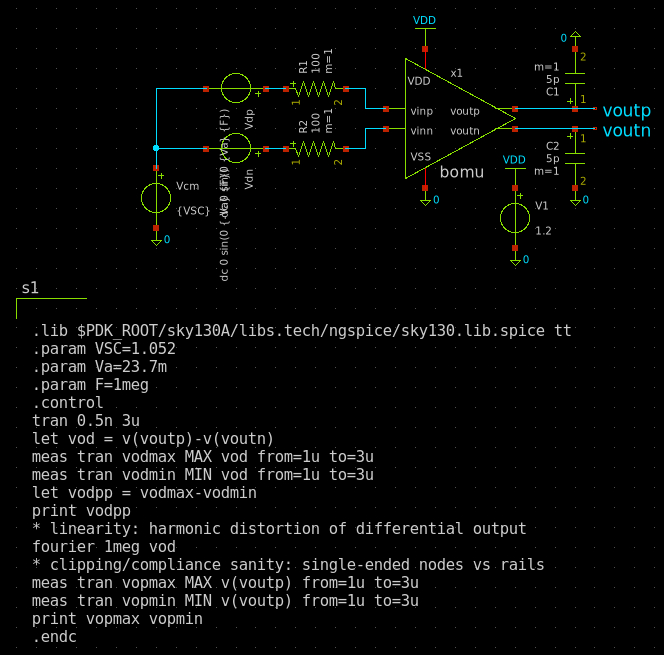
\includegraphics[width=12cm]{Figures/Xschem_Output_Swing_TB.png}
\caption{The transient swing testbench \texttt{ip/tb\_bomu\_swing.sch}.}
\label{fig:swingtb}
\end{figure}

\paragraph{Third-harmonic dominance.} A Fourier decomposition of $v_{od}$ (fundamental
$1MHz$, ten harmonics) gives $\text{THD}=0.53\%$, set almost entirely by the third
harmonic (Table~\ref{tab:thd}). Two features are characteristic of a balanced
source-coupled pair. First, the even harmonics vanish (at the $\sim10^{-14}$ numerical
floor): even-order distortion is common-mode and cancels in
$v_{od}=v(\text{voutp})-v(\text{voutn})$, so their absence confirms the devices and
loads are symmetric. Second, the residual distortion is odd-order, led by the third:
the large-signal transfer $i_{od}\propto\tanh\!\big(v_{id}/2nV_T\big)$%
\footnote{The tanh is exact for a differential pair whose devices follow the
moderate/weak-inversion exponential law $i_D\propto\exp(v_{GS}/nV_T)$. With
$V_T=kT/q$ the thermal voltage and $n$ the subthreshold slope factor.} is an odd,
compressive function whose Taylor expansion carries only odd powers, so the cubic term
folds back as a third harmonic. The fifth and higher harmonics fall off by orders of
magnitude, hence $\text{THD}\approx$ the third-harmonic term alone. Because that term
scales with the cube of the drive, distortion climbs quickly with swing; at the
$400mV_{pp}$ operating point it stays a clean $0.53\%$.

\begin{table}[H]
    \centering
    \caption{Fourier spectrum of $v_{od}$ at the $391mV_{pp}$ operating point
             (\texttt{tt}, $1.2V$, $27^\circ$C, $1MHz$ drive).}
    \label{tab:thd}
    \begin{tabular}{c|c|c|l} \hline
        Harmonic & Freq [MHz] & Norm. mag & \\ \hline
        1 & 1 & $1.000$ & fundamental ($0.197\,V$ ampl.) \\ \hline
        2 & 2 & $3\times10^{-14}$ & even (cancelled) \\ \hline
        3 & 3 & $5.3\times10^{-3}$ & dominant ($\approx$ THD) \\ \hline
        4 & 4 & $2\times10^{-14}$ & even (cancelled) \\ \hline
        5 & 5 & $3.6\times10^{-6}$ & \\ \hline
        7 & 7 & $1.8\times10^{-7}$ & \\ \hline
    \end{tabular}
\end{table}

\section{Small-Signal Quality: Offset, CMRR, PSRR and Noise}
\label{sec:quality}
Beyond the headline gain/bandwidth/swing targets, the pair was characterized for
input offset, common-mode and supply rejection, and noise, at \texttt{tt}/$1.20V$/
$27^\circ$C via \texttt{sim/corners.py mc} and \texttt{sim/corners.py acq}. One
caveat frames every mismatch-dependent number: sky130A's open \texttt{ngspice} models
carry mismatch slopes but never apply them (no
\texttt{agauss}/\texttt{mc\_mm\_switch} term in the model expressions, and the device
subckt ignores \texttt{delvto}), so there is no native statistical Monte Carlo.
Mismatch is therefore injected with a Pelgrom model using an assumed
$A_{VT}=4mV\!\cdot\!\mu m$. The absolute offset/CMRR/PSRR figures scale with that
coefficient and should be re-run against a measured $A_{VT}$ for a more accurate calculations.

\paragraph{Input offset.} A $200$-draw Monte Carlo (per-device $V_{th}$ offset plus
$0.5\%$ load-resistor mismatch, run as a single-invocation DC-op loop) gives
$\sigma(V_{os})=0.88mV$ ($3\sigma=2.65mV$, worst $2.,mV$), centred on zero. The
offset is small by construction: the pair is a
$W{=}320\mu m\times L{=}0.15\mu m=48\mu m^2$ device, so the Pelgrom term
$\sigma_{V_{th}}=A_{VT}/\sqrt{WL}=0.58mV$ per device ($\sqrt2$ for the pair gives
$0.82mV$). The large input devices that the sizing already demanded make offset a non-issue.

\paragraph{CMRR and PSRR.} Because the output is taken differentially between
matched halves, common-mode input and supply ripple couple almost entirely into the
output common mode and cancel differentially. The differential CMRR and
PSRR are matching-limited, not tail-limited, and are infinite for a perfectly
symmetric netlist. Evaluated at one $1\sigma$ mismatch draw they are
$\text{CMRR}=86dB$ and $\text{PSRR}=70dB$. The underlying common-mode paths set
the ceiling and are finite: the tail-limited common-mode gain is $A_{cc}=-17.8dB$,
and because $R_D$ couples $V_{DD}$ straight onto each drain the supply-to-common gain
is $A_{sc}=-10.7dB$. This is the same balance that suppressed the even harmonics in
Section~\ref{sec:swing}.

\paragraph{Noise.} The input-referred noise integrated over $10Hz$--$1GHz$ is
$47.9\mu V_{rms}$. Comparing against the $\sim34mV_{rms}$ input drive that produces
the $400mV_{pp}$ output swing, gives an input SNR of order $57dB$.

\begin{table}[H]
    \centering
    \caption{Small-signal quality at \texttt{tt}/$1.20V$/$27^\circ$C. Input offset
             and the differential CMRR/PSRR are mismatch-limited and scale with the
             assumed $A_{VT}=4mV\!\cdot\!\mu m$.}
    \label{tab:quality}
    \begin{tabular}{l|c|l} \hline
        \textbf{Metric} & \textbf{Value} & \textbf{Condition} \\ \hline
        Input offset $\sigma(V_{os})$ & $0.88$ mV & $200$-draw MC \\ \hline
        Input offset $3\sigma$ & $2.65$ mV & $200$-draw MC \\ \hline
        CMRR (differential) & $86$ dB & at $1\sigma$ mismatch \\ \hline
        PSRR (differential) & $70$ dB & at $1\sigma$ mismatch \\ \hline
        Common-mode gain $A_{cc}$ & $-17.8$ dB & tail-limited \\ \hline
        Supply$\rightarrow$CM gain $A_{sc}$ & $-10.7$ dB & $R_D$ direct coupling \\ \hline
        Input-referred noise & $47.9\mu V_{rms}$ & $10Hz$--$1GHz$ \\ \hline
    \end{tabular}
\end{table}

\section{Status and Next Steps}
\label{sec:status}
The central result (Section~\ref{sec:sweeps}) is that the $10dB$ / $150MHz$
specification sits on the single-stage gain--bandwidth wall $g_m/(2\pi C_L)$, which
nominal clears by only $\sim1.5\%$. A small $g_m$ increase and a $\sim7\%$
parasitic margin give a nominal-passing $W=78\mu m$ point, but PVT sign-off
(Section~\ref{sec:corners}) fails the full $63$-corner box, forcing a re-size to
$W=320\mu m$ / $R_D=193\Omega$ under a regulated-$1.20V$ rail. At that point the
schematic passes $61/63$ ($21/21$ regulated). The block is laid out LVS/DRC-clean
(Section~\ref{sec:layout}), and the parasitic-extracted (RCX) netlist re-run across
all $63$ corners (Section~\ref{sec:pex}) reproduces a uniform
$\sim-3.7\%$ bandwidth, $\sim0dB$ gain penalty with all $21$ regulated-rail points
passing. The signed-off GDS and reports are in \texttt{tapeout/}.

Remaining / optional work:
\begin{enumerate}
    \item The two marginal PVT misses ($9.6$--$9.8dB$ at $-5\%V_{DD}+$hot$+$low-$R$)
          are the single-stage GBW wall, not a trim: closing them for a symmetric
          $\pm5\%$ supply would need either a relaxed $\sim9dB$ gain spec, a higher
          nominal rail ($\sim1.25V$), or a topology change.
    \item \texttt{sim/tb\_ac.spice} is a single-point AC demonstration deck at the
          pre-PVT nominal ($W=78\,\mu m$) point. The only remaining
          idealisation is that its $R_{ref}$ uses a round value rather than the
          extracted \texttt{res\_high\_po} resistance, which could be trimmed for an
          exact match, however, this would be mostly cosmetic as both sims already match closely.
\end{enumerate}

\bibliographystyle{IEEEtran}
\bibliography{Sources}

\end{document}
